\subsection{Analysis of Vulnerable domains}

We performed the following analyses on the vulnerable domains:
\begin{itemize}
	\item Checking Alexa rankings of the vulnerable domains.
	\item Investigating the back-end languages used by the vulnerable domains.
	\item Analyzing the presence of DKIM (DomainKeys Identified Mail), SPF (Sender Policy Framework), and DMARC (Domain-based Message Authentication, Reporting \& Conformance) mechanisms on these domains.
\end{itemize}


\subsubsection{Alexa rankings of vulnerable domains.}
We searched through the Alexa rankings data\cite{alexa} for the domains that were found to be vulnerable, and found 135 of these domains in the top 1 million ranked websites. A detailed distribution of the rankings is shown in Table~\ref{tab:alexa} / Figure~\ref{fig:alexa_data_bar} / Figure~\ref{fig:alexa_data_pie}.

%TODO Adam: Need to decide if table or graph, if graph, then Pie vs Bar.
%\begin{table}[tbp]
%	\centering
%	\scriptsize
%	\begin{tabular}{|l|c|}
%		\hline
%		\textbf{Alexa Ranking Ranges} & \textbf{Vulnerable domains} \\
%		\hline
%		0-5K & 1 \\
%		\hline
%		5-50k & 7 \\
%		\hline
%		50k-100k & 6 \\
%		\hline
%		100k-250k & 23 \\
%		\hline
%		250k-500k & 30 \\
%		\hline
%		500k-1m & 68 \\
%		\hline		
%	\end{tabular}
%	\caption[\titlecap{Distribution of vulnerable domains based on Alexa Rankings}]{Distribution of vulnerable domains based on Alexa Rankings}
%	\vspace{-5ex}
%	\label{tab:alexa}
%\end{table}

\begin{figure}
	\centering
	\begin{minipage}{.5\textwidth}
		\centering
		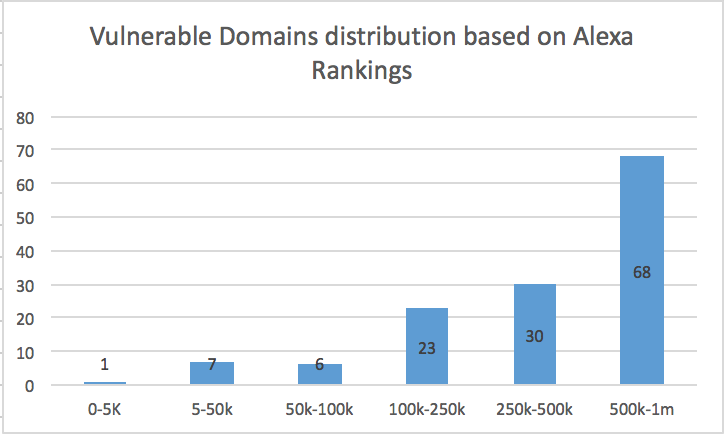
\includegraphics[width=.95\linewidth]{alexa_data_bar}
		\captionof{figure}{Distribution of vulnerable domains based on Alexa Rankings}
		\label{fig:alexa_data_bar}
	\end{minipage}%
	\begin{minipage}{.5\textwidth}
		\centering
		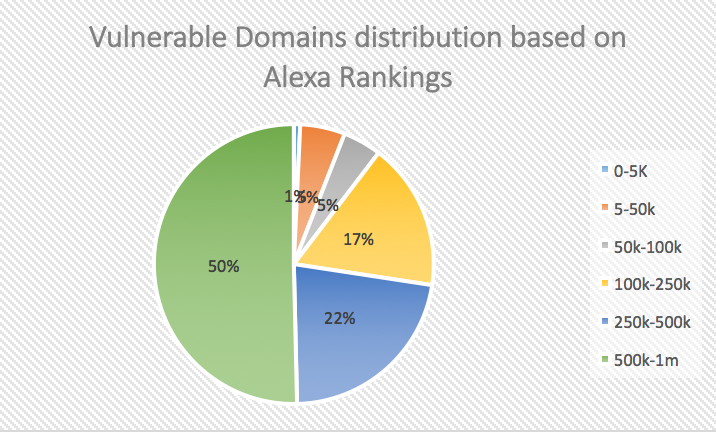
\includegraphics[width=.95\linewidth]{alexa_data_pie}
		\captionof{figure}{Distribution of vulnerable domains based on Alexa Rankings}
		\label{fig:alexa_data_pie}
	\end{minipage}
	\vspace{-1.5ex}
\end{figure}

\subsubsection{Back-end languages of vulnerable domains.}
\subsubsection{Presence of e-mail spoofing protection on vulnerable domains.}